\section{Introduction}
Natural Language Inference (NLI), also known as the Recognizing Textual 
Entailment (RTE) is a task of determining whether a text premise $p$ 
can entail, contradict or be neutral with a given hypothesis $h$~\citep{DBLP:conf/mlcw/DaganGM05}. 
This task servers as an important benchmark for testing model's reasoning 
ability.
% It's also widely used as an invaluable aid in other NLP tasks, such as dialogue consistency~\citep{DBLP:conf/acl/WelleckWSC19}.

Although NLI is proposed as a classification problem, 
it's also worth considering it as a generation task. Recently, 
several works reformulate NLI task as a generation task~\citep{DBLP:journals/corr/KolesnykRR16,DBLP:journals/csl/StarcM17,DBLP:journals/corr/abs-1803-02710,DBLP:journals/corr/abs-1909-09788}. 
They explore how to generate the hypothesis $h$ given 
a premise $p$ and a logic condition $c$ or reversely generate $p$ given $h$ and $c$. 
\citet{DBLP:journals/corr/KolesnykRR16} show that the task of generating 
entailed sentences can be served as a benchmark to measure the reasoning 
ability of sequence to sequence models.
\citet{DBLP:journals/csl/StarcM17} first use it for data augmentation. They use generated hypotheses to construct a new NLI style dataset, on which a better classifier can 
be trained.

\begin{figure}[t]
	\centering
	\scalebox{1.0}{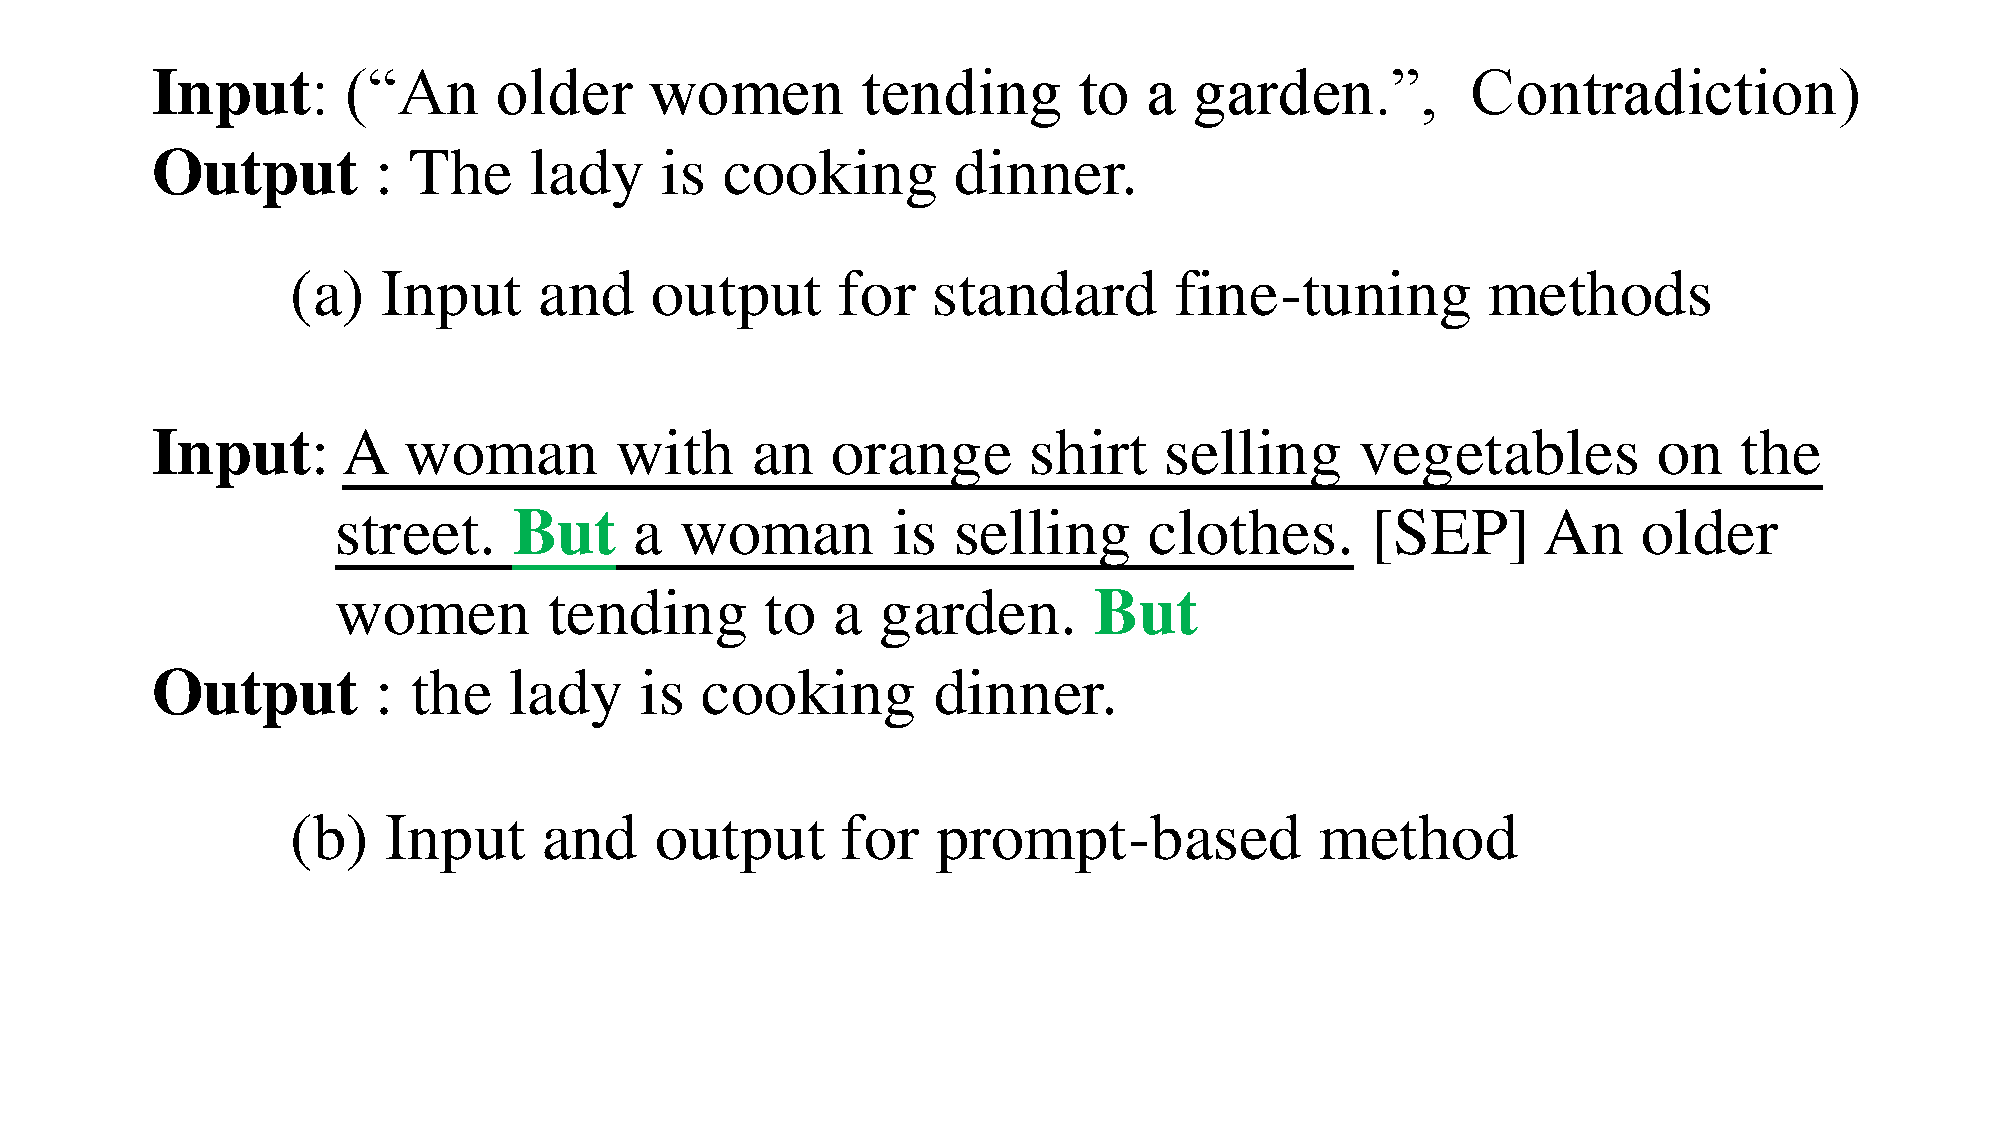
\includegraphics[width=1.0\columnwidth]{figure/intro_prompt.pdf}}
	\caption{The difference between how standard fine-tuning methods and prompt-based methods treat the NLI generation task. The underlined text is a demonstration. The Green words are condition-specific templates.} \label{fig:intro_prompt}
\end{figure}

However, the success of these works heavily depends on the 
SNLI dataset~\citep{DBLP:conf/emnlp/BowmanAPM15}, which is a manually created 
dataset. Thus it's a challenge to use the proposed approaches in specific domains or real-world applications which are different from the SNLI domain, 
and where there is not enough annotated data. In light of this, 
we want to explore how to improve the performance of NLI generation task 
in a few-shot setting.

Recently prompt-based learning has led to large improvements in NLP tasks under zero-shot or few-shot settings~\citep{liu2021pre,DBLP:conf/emnlp/PetroniRRLBWM19,DBLP:conf/eacl/SchickS21,DBLP:conf/emnlp/ShinRLWS20}. The main idea is to reformulate the downstream tasks as the pre-training task of pre-trained Language models (PLMs) using a prompt template. \citet{DBLP:conf/nips/BrownMRSKDNSSAA20} show that given a few demonstrations of inputs along with the prompt, GPT-3 achieves near state-of-the-art results in some SuperGLUE tasks.
Inspired by their success, we investigate how to adapt prompts and demonstrations to NLI generation task, which is reformulated as shown in \figref{fig:intro_prompt}(b).

Finding the right prompt is the first stage. 
% \citet{DBLP:conf/acl/GaoFC20} proposed to use the generative T5 model~\citep{DBLP:journals/jmlr/RaffelSRLNMZLL20} to automatically generate a lot of candidate templates. Then measure the performance for each template on development set to choose the best one. 
The problem of generating candidate templates and choosing the best one on the development set method proposed by \citet{DBLP:conf/acl/GaoFC20} is that in NLI generation task, we need to induce different templates for different conditions which makes the result on the development set less reliable,  
since we only use a subset of the data to measure each template. 
To ameliorate this, we propose a max-margin strategy to pick the template that 
receives a high score in its corresponding condition but low scores 
in all other conditions, considering the conditions in NLI task are conflicting with each other.

The second stage is to sample demonstrations. \citet{DBLP:conf/acl/GaoFC20} and \citet{DBLP:journals/corr/abs-2101-06804} simply sample them by the static cosine similarity based on models trained on related datasets (this model is regarded as a \textit{retriever}). This approach is suboptimal as: 
(1) it doesn't make use of the training data;
(2) in cases of a low-resource language, we 
do not have sufficient labeled data to train such a retriever.
To address these issues, 
we propose a dynamic method that combines 
the probability from the generator and the probability from the retriever to help the retriever fit target tasks.

In summary, our contributions are:
(1) To the best of our knowledge, we are the first to investigate NLI generation task in a few-shot setting.
(2) We propose a max-margin template selection method and a dynamic 
demonstration selection method. Combining these two methods with PLMs, 
our LM-PDD model gains 8\% absolute improvement over the standard fine-tuning models.
(3) We test our demonstration selection method on 
13 natural language classification tasks in few-shot settings, 
the results show our method has strong generality.

%Our experiments show in a few-shot setting, (1) prompt-based methods outperform standard fine-tuning methods. (2) the template chosen by the scores in all conditions outperforms the one chosen by score in one condition. (3) training the retriever together significantly improve the performance. Combining these methods together our model gains 13\% improvement compare to standard fine-tuning methods, which provides a possible way to perform NLI generation in a few-shot scenario. Finally we test the generalization ability of our methods on 13 different natural language classification tasks. The result shows our method works for a wide range of NLP tasks.
